\documentclass[letterpaper, 11pt]{article}
\usepackage[hyperref]{acl}\aclfinalcopy
\usepackage{times}
% adapted from https://tex.stackexchange.com/a/338931/19048

\usepackage{collcell}
\usepackage{hhline}
\usepackage{pgf}
\usepackage{multirow}

\def\colorModel{hsb} %You can use rgb or hsb

\newcommand\ColCell[1]{
  \pgfmathparse{#1<50?1:0}  %Threshold for changing the font color into the cells
    \ifnum\pgfmathresult=0\relax\color{white}\fi
  \pgfmathsetmacro\compA{0}      %Component R or H
  \pgfmathsetmacro\compB{#1/100} %Component G or S
  \pgfmathsetmacro\compC{1}      %Component B or B
  \edef\x{\noexpand\centering\noexpand\cellcolor[\colorModel]{\compA,\compB,\compC}}\x #1
  } 
\newcolumntype{E}{>{\collectcell\ColCell}m{1.5cm}<{\endcollectcell}}  %Cell width
\newcommand*\rot{\rotatebox{0}}

\usepackage{latexsym,booktabs,colortbl,todonotes}
\usepackage{graphicx}

\usepackage{geometry}
\geometry{margin=0.6in}

% \graphicspath{ {./images/} }
\usepackage{mathtools,amsmath}
\DeclareMathOperator*{\argmax}{arg\,max}
\DeclareMathOperator*{\argmin}{arg\,min}
\DeclarePairedDelimiter\ceil{\lceil}{\rceil}
\DeclarePairedDelimiter\floor{\lfloor}{\rfloor}

\begin{document}
\title{
    COMP 551 - Mini-Project 2
}
\author{
    Orla Mahon, Lambert De Monte, Jacob Louis Hoover
}

\date{\today}

\maketitle

\thispagestyle{empty}
\pagestyle{plain}
%%%%%%%%%%%%%%%%%%%%%%%%%%%%%%%%%%%%%%%%%%%%%%%%%%%%%%%%%%%%%%%%%%%%%%%%%%%%%%%%
\begin{abstract}
The task we tackled for this mini-project was to develop and compare models to analyze comments from the website Reddit and to predict from which of the site's communities a given comment originated. We developed our own implementation of the Bernoulli Na\"ive Bayes Algorithm from scratch and compared it to various models available in the scikit-learn package in terms of accuracy and runtime. We also performed text pre-processing methods dataset prior to running the models in order to reduce the feature space, and increase accuracy. Our key finding from this project was that a soft voting ensemble method of several different underlying classifiers was more accurate than any individual model on its own. 

\end{abstract}
%%%%%%%%%%%%%%%%%%%%%%%%%%%%%%%%%%%%%%%%%%%%%%%%%%%%%%%%%%%%%%%%%%%%%%%%%%%%%%%%
\section{Introduction}

For this project, we were assigned the task of building or implementing models to identify which of a set of possible Reddit communities a user comment had originated from. The dataset of both training and testing comments that we were given were evenly distributed between the 20 possible Reddit communities and we performed pre-processing on it in order to decrease the amount of feature space and to improve the accuracy of our models' predictions. 

There were two main steps to our method in this project, the first of which was to implement our own Na\"ive Bayes Algorithm without the use of external packages, which including developing a \texttt{fit} method to generate the matrix of probabilities and a \texttt{predict} method to map this matrix to a test set of comments in order to generate the category predictions for each one. The second main step was to implement various other models using scikit-learn's packages, in order to see which one performed the best for this task. 

Our best individual model was the scikit-learn Complement NB model, which achieved an accuracy of about $56\%$.  Other scikit-learn models achieved similar accuracy. However, it was using an ensemble method with a confidence-weighted majority vote that we achieved our best accuracy, getting 58\% on our local tests (57.955\% on the Kaggle competition's public leader board).

Some of our other discoveries during this project were that the \texttt{WordNet} Lemmatization was less effective than the \texttt{PorterStemmer} in terms of final prediction accuracy, and that an individual model by itself may do fairly well with its predictions, but an ensemble method that pools their results is even more accurate still. Within these voting methods, we also found that a 'soft' vote, where the predictions are averaged, fared better than a 'hard' vote, where the predictions are reduced to a binary form. 

\subsection*{Related work}

Text classification is a popular topic for machine learning applications, and a multitude of studies investigate tasks similar to the task we attempted, where the goal is to classify text samples into classes or categories which can be assigned by humans.\cite{Boiy:2009} While our project's setup is similar to these, it is also somewhat different as both our training and our testing datasets are made up of comments taken from a variety of Reddit communities, each of which was specifically chosen by a user who decided to reply within it. 

Other studies have looked more in depth at the pre-processing phases of Machine Learning, for instance \cite{Sharma:2015} found that the two most important pre-processing techniques that affect feature selection are the process of stemming---to standardize words with similar stems, and the removal of stop words---generic, common, and purely grammatical words that have little effect on the categorization of a phrase. Helpfully, these techniques both also have the effect of reducing the number of features used in later stages of their experiment, though only by a relatively small amount (the feature vectors based on counts/occurrences of words are still sparse vectors in high-dimensional space). 

Another study examined the impact of using datasets that contained spelling and grammar irregularities, which are fairly common in blog-style websites like Reddit, and are known as 'noisy' or 'dirty' datasets.\cite{allstate} By using both Stemming and Lemmatization, they were able to build a high accuracy prediction model, with both categories and comments classified as 'noisy'. In our project, it is only the comments which will be noisy, and we found that using lemmatization, whether with or without stemming did not provide a large boost in performance.

While Na\"ive Bayes has generally been found to be less accurate than Support-Vector Machines\cite{twitterNB}, many studies have found that Multinomial\cite{MNBvsNB} or Complement Na\"ive Bayes\cite{Seref:2019} are more effective with regards to precision and accuracy of predicted results, a generalization that was reflected in our results.  

%%%%%%%%%%%%%%%%%%%%%%%%%%%%%%%%%%%%%%%%%%%%%%%%%%%%%%%%%%%%%%%%%%%%%%%%%%%%%%%%
\section{Datasets}

Both the testing and training datasets were made up of comments from 20 different categories (called `subreddits'), with the number of comments originating from each evenly distributed between the categories.  The training set (70k comments) had category of each comment labelled, while for the test set (30k comments), the correct labels were held out for testing in the Kaggle competition.

\subsection{Pre-processing}
After parsing the comments, we ran a short gamut of text cleaning functions.  First, we chose a list of symbols to treat as delimiters (replacing any instances of the characters \texttt{\textbackslash/()\{\}[]\textbar@,;} with a space) after which we removed any other non-alphanumeric characters (except \texttt{\_+\#}). We then used nltk's list to delete English stopwords. The point of this cleaning was to make the content of the comments be more heavily content words, that is, words which should be on average more likely to be indicative of the category.

After cleaning, we used nltk's word tokenization, and the \texttt{PorterStemmer}  (which we found more effective than \texttt{LancasterStemmer}) in order to standardize each comment's words, removing any prefixes, suffixes, and endings which did not affect the core meaning of a word, the purpose for this stemming being to consolidate words with nearly identical meanings into a single feature. Lemmatization would have theoretically been a stronger version of this process (as it works to unify words with similar meanings, even if they are not etymologically related), and we did try downloading WordNet and using the WordNet lemmatizer, but we found it to be less effective than the PorterStemmer on the downstream classification task in this case. 

After cleaning and stemming, we had a total of about 70,000 different words in our entire corpus of test comments.  In the following, we can refer to this set of words as our \textbf{vocabulary}.

%%%%%%%%%%%%%%%%%%%%%%%%%%%%%%%%%%%%%%%%%%%%%%%%%%%%%%%%%%%%%%%%%%%%%%%%%%%%%%%

\section{Proposed approach}
 

\subsection{Extracting features---our pipeline}
We set up a basic pipeline on which to test various scikit-learn models, and tune hyperparameters.  This pipeline consisted of first extracting usable features from the comments, using a count vectorizer, and then transforming those features to tf-idf scores, before passing the result into a given model.  Each of these transformers is described briefly below:

\paragraph{\texttt{CountVectorizer}} This transformer maps each text comment to a set of features by simply counting the occurrence of each word from the vocabulary (so each comment becomes a sparse vector of number of dimensions equal to the size of the vocabulary). We also played with the possibility of only considering the $k$ most common words in the vocabulary, since most words in the 'long tail' are not very informative. This $k$ was a hyperparameter we experimented with, but most of our models had higher slightly higher accuracy when $k=$ size of full vocabulary, though performance was slightly slower.

We also experimented with using \textbf{$n$-grams} as features (using as features  $n$ adjacent words, rather than just one word).  We played with using only single word features, using single words as well as bigrams, and using only bigram features.  In the end (perhaps somewhat surprisingly) using bigrams never improved our performance.

\paragraph{\texttt{TfidfTransformer}} This transformer takes the count vector from the previous step and changes them to reflect the proportional to the number of documents in which that word appeared.  While including this transformation did not make a large difference it only ever boosted performance.

After applying the above two transformers the feature vector is fed into the model of choice (choosing among a number of sklearn models as well as our hand-coded Na\"ive Bayes model). 

\subsection{The models}\label{subsec:the-models}

The first model to mention is the Bernoulli Na\"ive Bayes classifier, which we implemented manually (with python's numpy, and scipy's sparse matrix packages for the linear algebra), and attempted to minimize the use of loops in favour of matrix operations for faster run-times. In the end, however, this model was not among the stronger models compared to the out-of-the-box scikit-learn models which we used in attempting to achieve the best possible classification accuracy.

We experimented with a number of sklearn's classifier models, and found that we could achieve relatively good accuracy with Bernoulli, Multinomial, and Complement Naïve Bayes, a SGD Classifier, LinearSVC, K-Nearest Neighbours, Logistic Regression, Random Forest, and Passive Aggressive Classifier.  Each of these classifier models of course has hyperparameters to set, and so for each model we wished to optimize, we used sklearn's \texttt{GridsearchCV} to search for hyperparameters using the following setup:  we first split the 70k comments from the provided training data into a 70\%-30\% train-validate split, and we then fed that training split into a GridsearchCV model, which used 5-fold cross validation to find the best set of parameters, from a set of hyperparameter values we would choose. We then fit the resulting best model on the entire train split, and measured accuracy by predicting on the 30\% validate split. We then retrained our final model on the whole training set before making predictions on the held out competition set.

We also debated using sklearn's Linear Discriminant Analysis and Quadratic Discriminant Analysis models, as it would have been interesting to see how these solutions would have fared in terms of accuracy, especially given that they have no hyperparameters to tune, unlike the other models. However, due to a lack of processing power and memory space in our respective personal computers, we were forced to abandon this idea. 

\subsection{Ensemble Method}
We tried using a voting classifier, an easy method to start experimenting with aggregating multiple models to get a better prediction. For this classifier, the choice of which models to include as predictors is one meta-hyperparameter (each of the models  that are included of course having their own hyperparameters), the other hyperparameter of this model being the choice of `hard' vs `soft' voting.

A soft voting classifier gets the category label predictions based on the maximum value of the sums of the probabilities predicted by the different predictor models in the ensemble (selecting category to which the models together gave the most probability mass), while a hard voting classifier, simply solicits a binary response from each model's prediction, and selects the category with by majority vote.

We also tried an implementation of a boosting algorithm, AdaBoost, which and implements multiple (say, $k$) copies of a given base `weak' classifier, and iterates through, making predictions, and successively adding weak classifiers to the total classifier, subject to a weighting scheme based on the accuracy of the weak classifier, with examples that are misclassified being given more weight in subsequent iterations. This model has been shown to be capable of building a much stronger classifier from a set of weaker classifiers. A decision tree classifier is a common choice for the weak classifier, but this boosting model can be implemented with a variety of classifiers as the weak classifier, and we experimented with this choice, as well as the hyperparameter $k$. However, we never managed to achieve accuracy at a level which made this model worth pursuing for our submission.


%%%%%%%%%%%%%%%%%%%%%%%%%%%%%%%%%%%%%%%%%%%%%%%%%%%%%%%%%%%%%%%%%%%%%%%%%%%%%%%%
\section{Validation and results}\label{sec:validation-results}

Initially, when evaluating the individual sklearn models, after playing with possible hyperparameter values for a while, we found that we could get passable results around 54--57\% accuracy (not too far below the TA baseline of 57\%) with a number of different models. Complement Na\"ive Bayes being the best (see the figure \ref{fig:complnb}, for confusion matrix), and Multinomial Na\"ive Bayes, Logistic Regression and other SGD models also faring roughly as well.
\begin{figure}
    \centering
    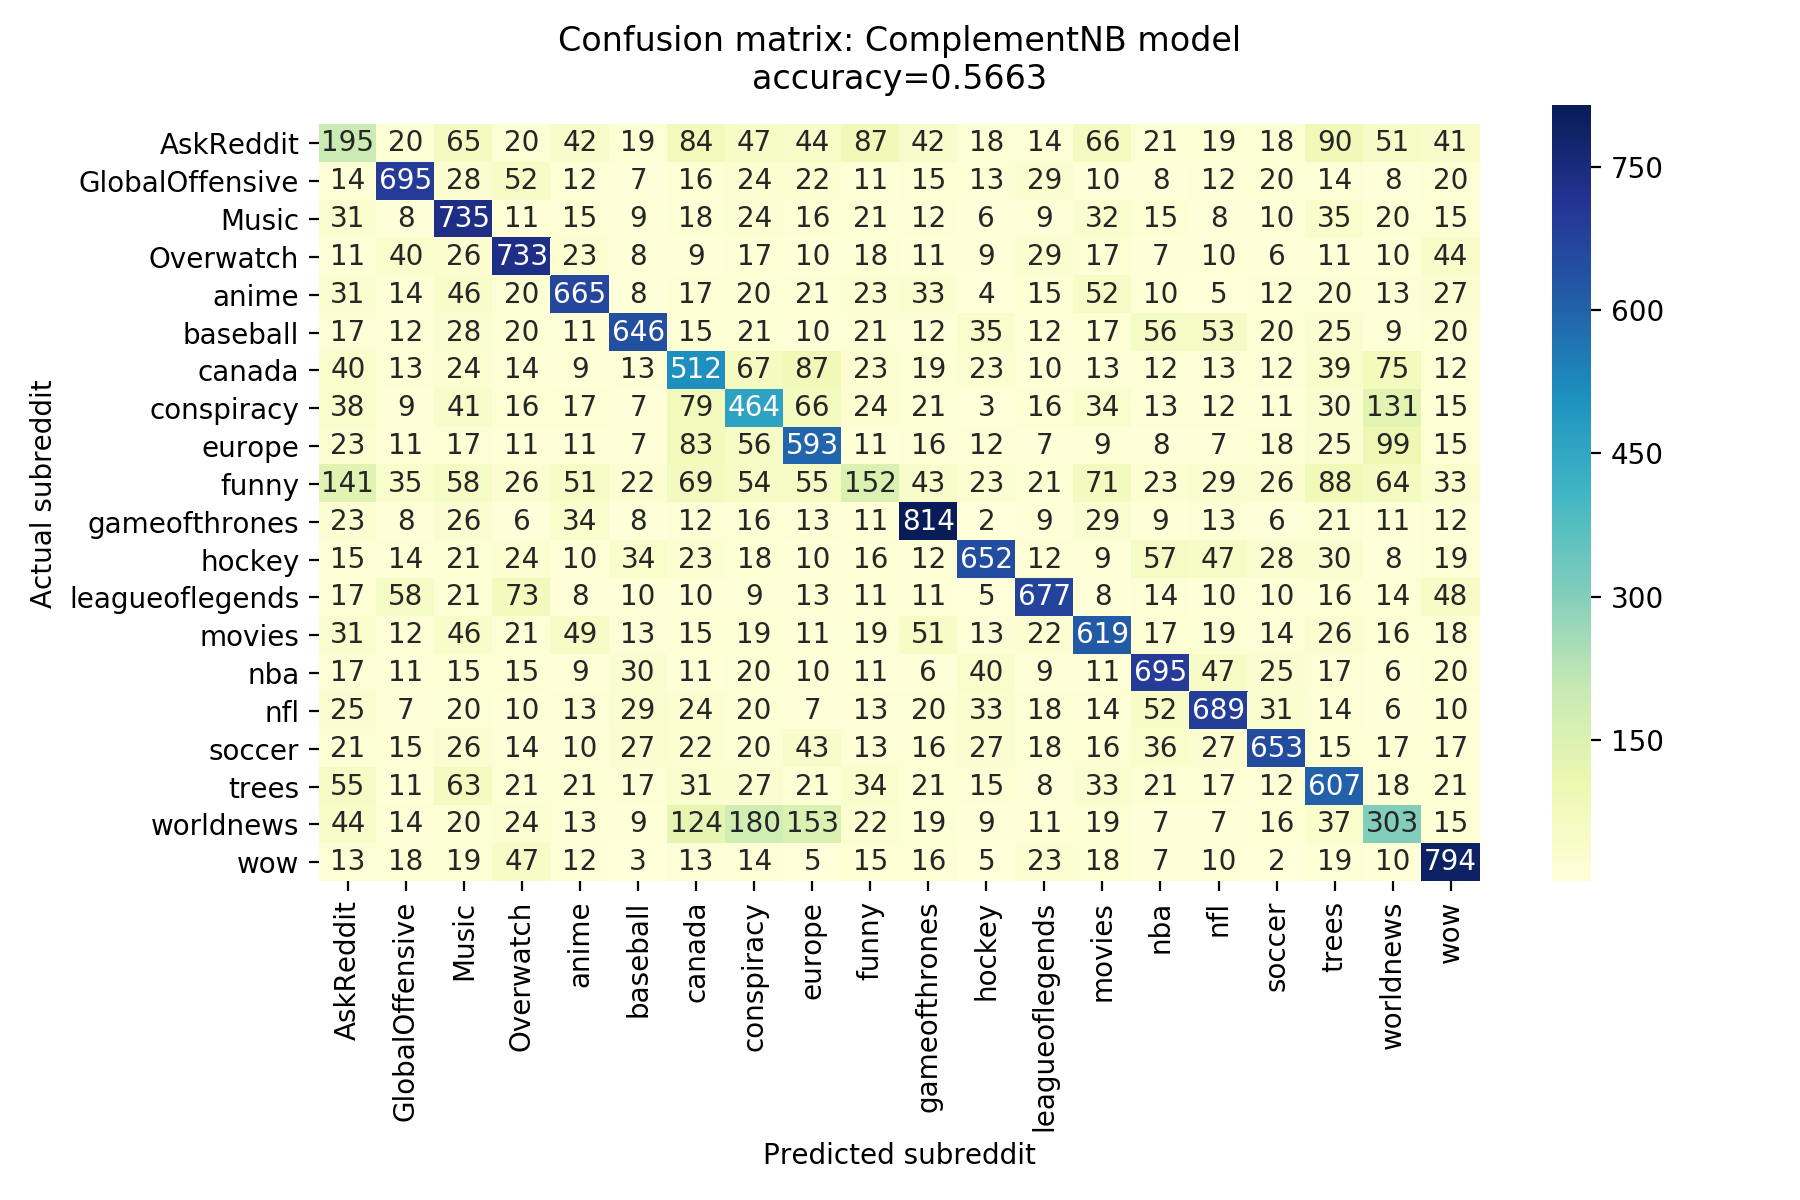
\includegraphics[width=\textwidth/2]{images/complementnb}
    \caption{Complement NB, the best individual model}
    \label{fig:complnb}
\end{figure}
\begin{figure}
    \centering
    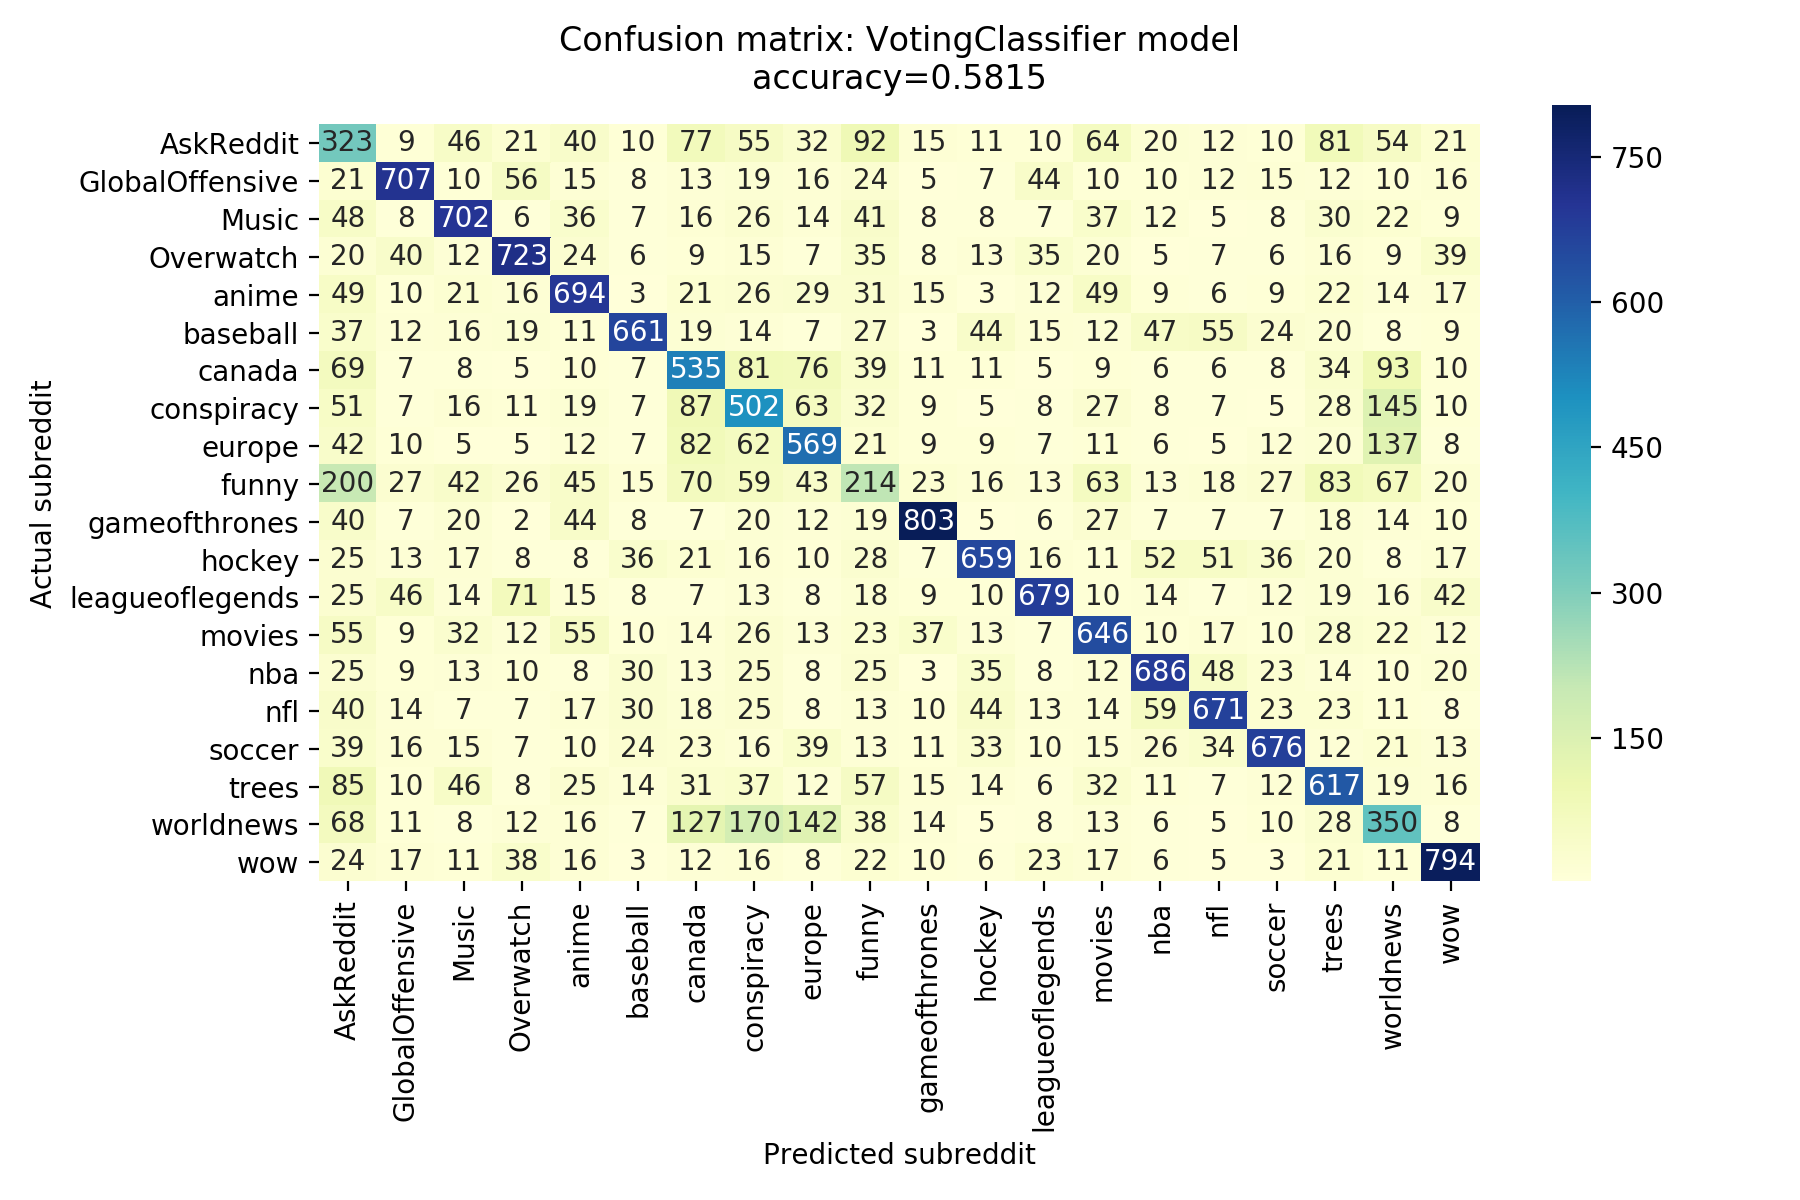
\includegraphics[width=\textwidth/2]{images/best-model}
    \caption{Soft voting classifier model over CNB, MNB, and LogReg.}
    \label{fig:votingclf}
\end{figure}

In order to boost performance, we tried implementing an some ensemble methods listed above.  The method which got us the best results was a voting classifier, we used GridSearch to play with various subsets of our 5 best-performing models as predictor models to make a voting classifier, trying both soft and hard-voting, and our best-accuracy model was a Soft Voting Classifier using Logistic Regression, Multinomial Na\"ive Bayes, and Complement Na\"ive Bayes.\footnote{Interestingly these were not quite the three highest-achieving models (the Logistic Regression model never was among the top three, and a hyperparameter for CNB which achieved best accuracy when part of the Voting Classifier was very different value from the value of that same hyperparameter when using CNB as a stand-alone classifier})

It was this soft voting classifier with which we made the predictions on the test set, to get our current best public leader-board accuracy of 57.955\% (which is slightly below the best accuracy achieved in our local tests with the same model: in our testing we measured an accuracy of 58.15 (see full confusion matrix: \ref{fig:votingclf})). 


The Bernoulli Na\"ive Bayes that we implemented manually was unfortunately one of our less successful models, we experimented with different values for our additive (Laplace) smoothing, and found that the best accuracy was achieved with a value of 0.01.  Our average best accuracy was around 30\% on this classification task. Evaluating Sci-kit learn's version of Bernoulli Na\"ive Bayes on the same number of features that we trained our version on (the 10,000 most commonly occurring words in our post-cleaning post-stemming vocabulary), we obtained a 48.5\% accuracy (Figure \ref{fig:bnb}). We suspect this disparity in accuracy between our model and the Sci-Kit Bernoulli Na\"ive Bayes may be related to the way we made use of sparse matrix operations within the prediction method of our implementation. Interestingly, our Bernoulli NB model had particular trouble with comments from \textbf{r/conspiracy}.\footnote{So, we might say, it really was a `na\"ive' model.} 

\begin{figure}
    \centering
    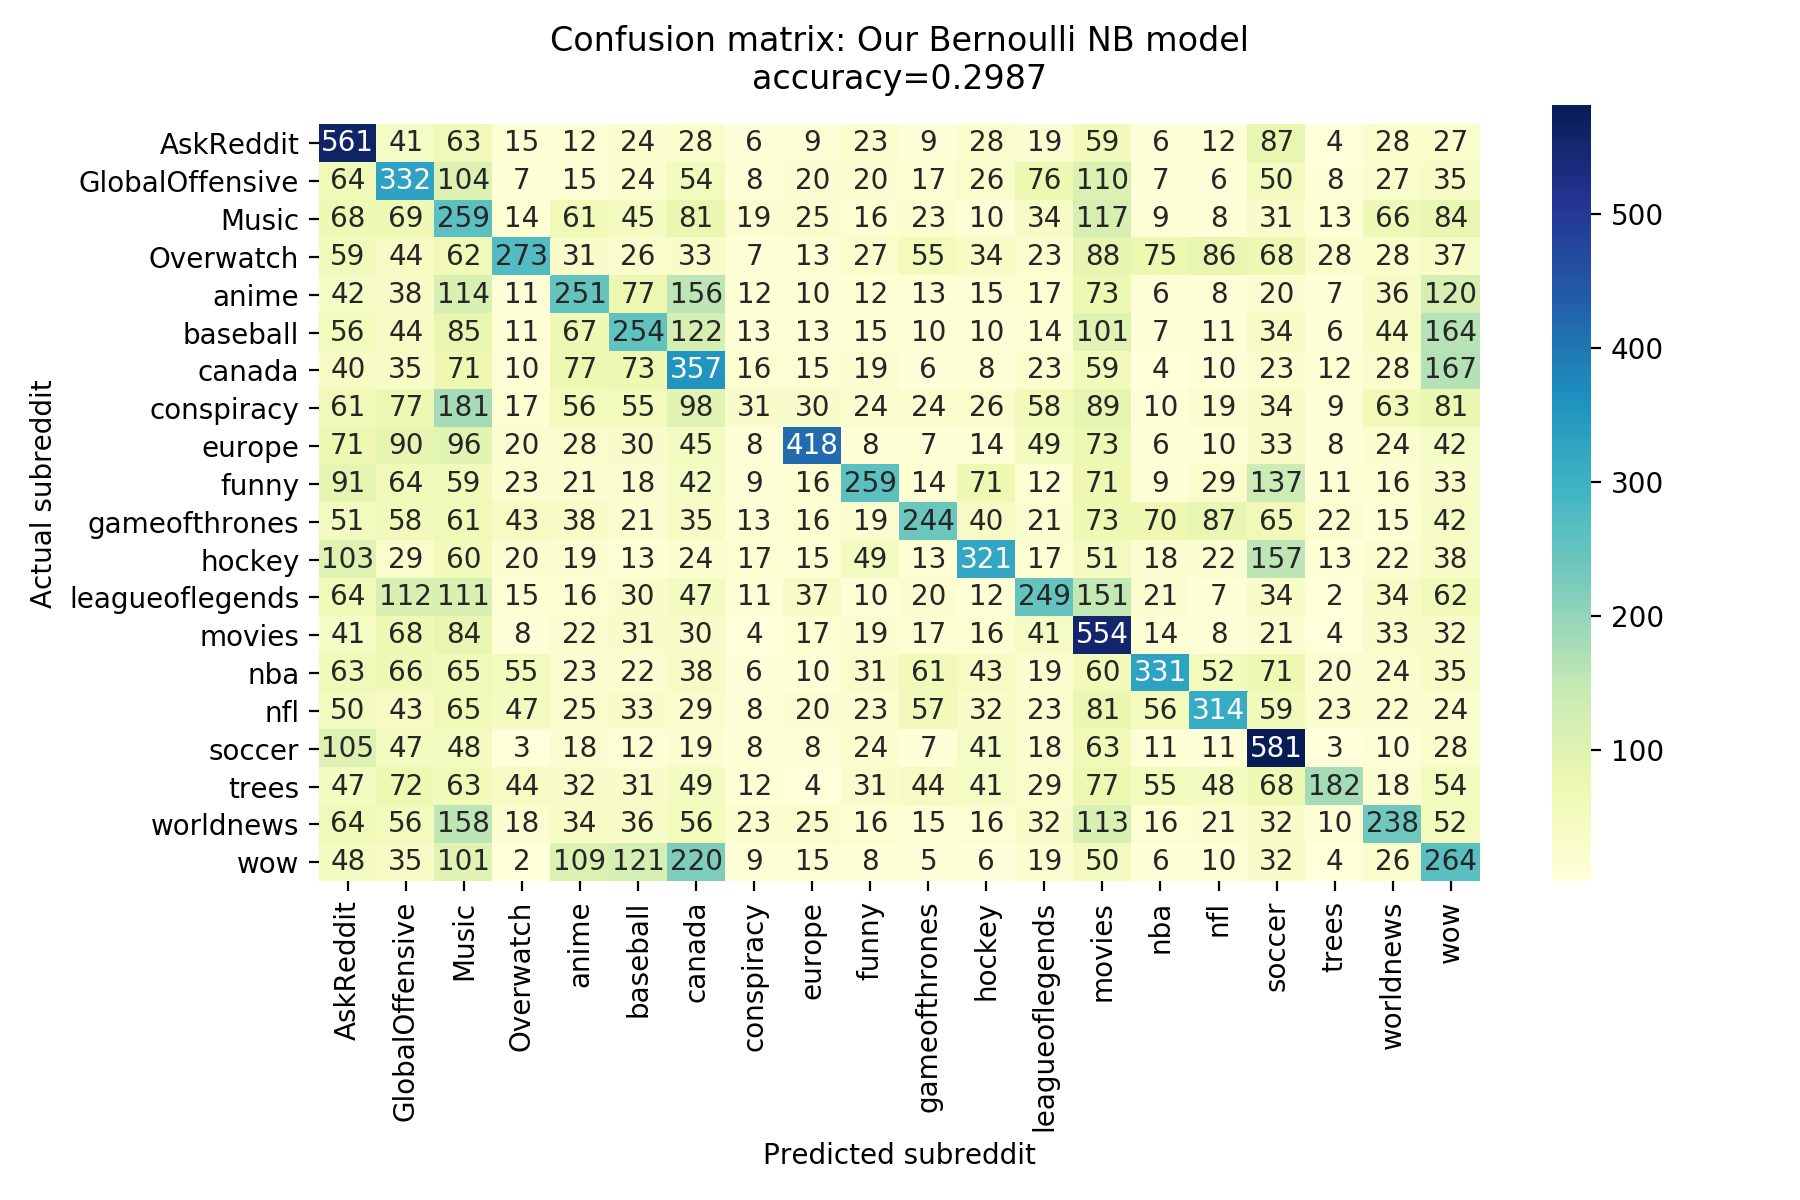
\includegraphics[width=\textwidth/2]{images/ourbernoulli}
    \caption{Our hand-coded Bernoulli NB model.}
    \label{fig:ourbnb}
\end{figure}   

\begin{figure}
    \centering
    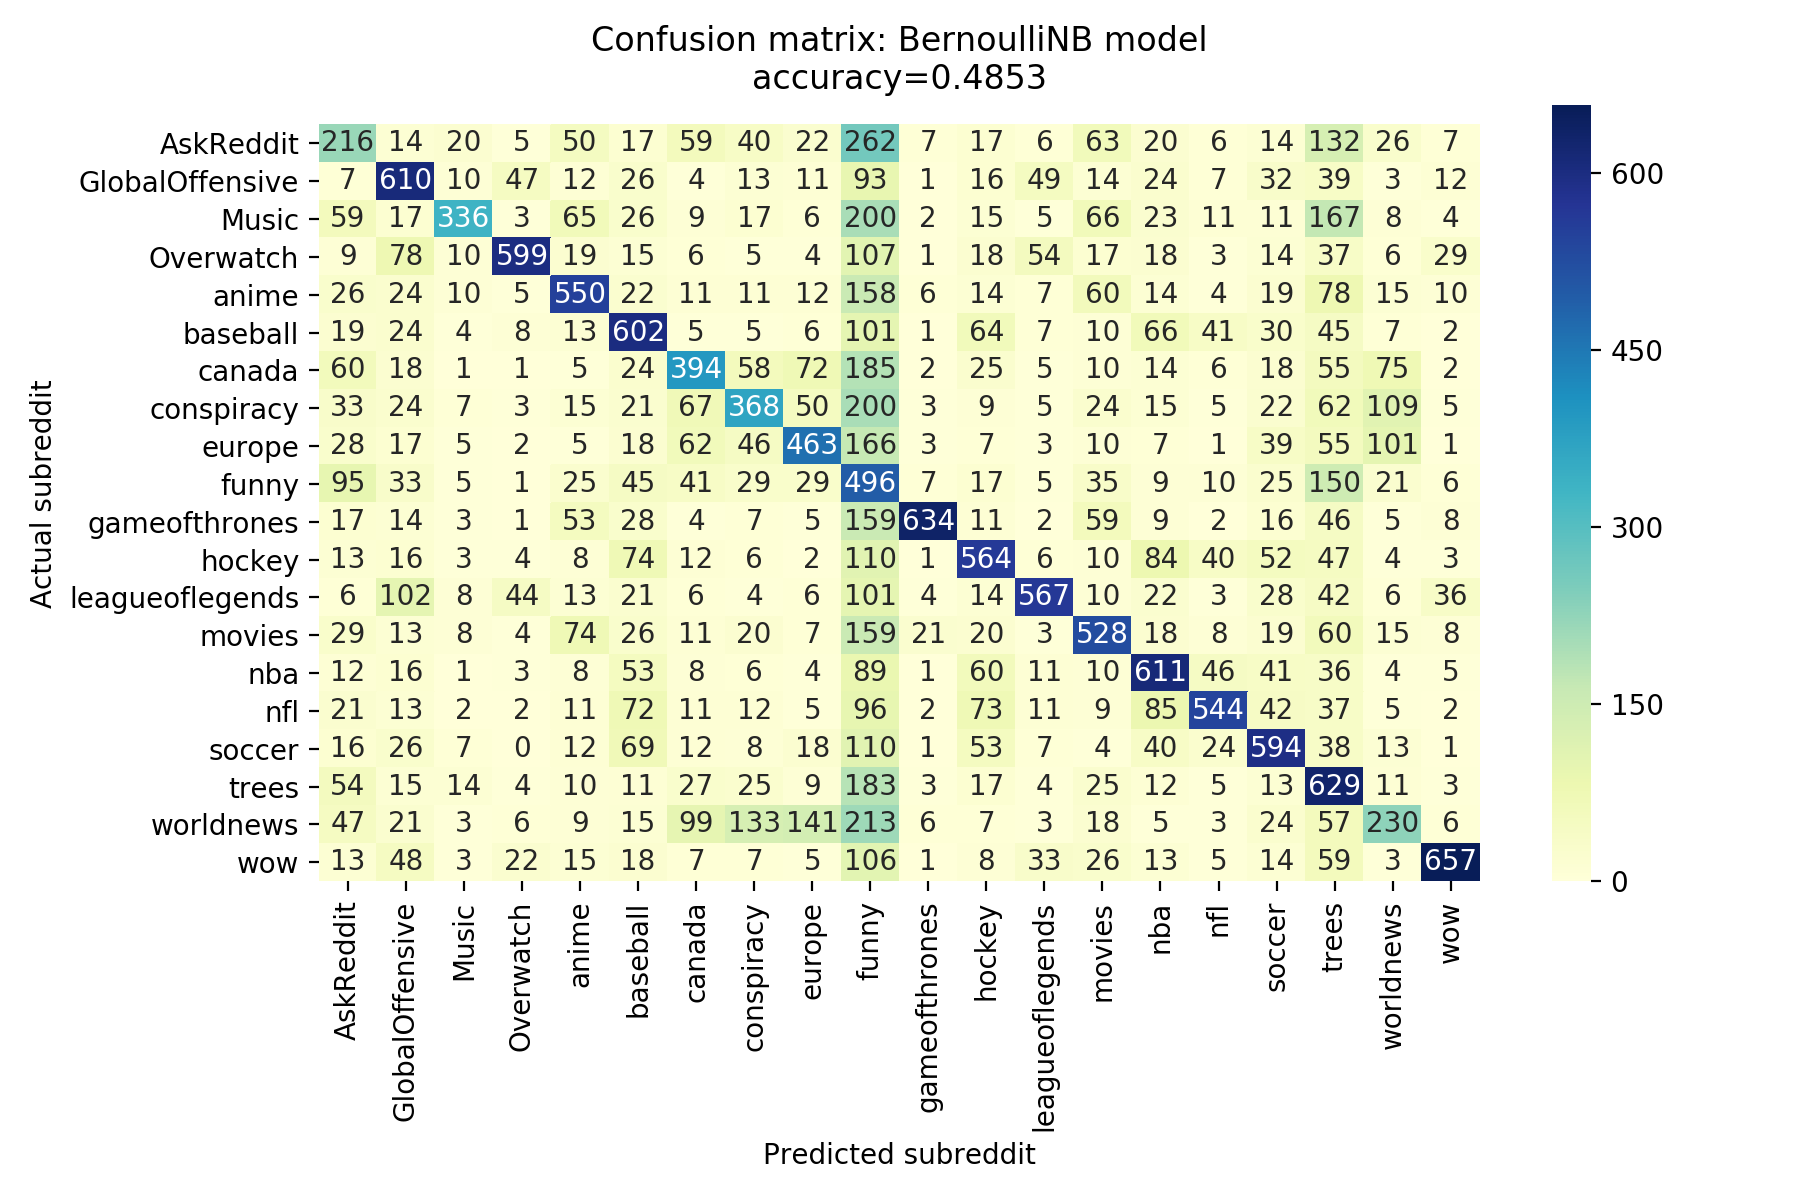
\includegraphics[width=\textwidth/2]{images/bnb}
    \caption{sklearn's Bernoulli NB model.}
    \label{fig:bnb}
\end{figure}

From the various Sci-Kit models we implemented, the one which reported the best individual accuracy was the Complement Na\"ive Bayes model, returning a 56\%.  

Something we noticed in our results is that most of the models we tested, with the exception of Bernoulli NB, had the most difficulty predicting comments which originated from the \textbf{r/funny} community. Our suspicion is that the models in general have difficulty predicting which comments would fall into the \textbf{r/funny} category because there is not necessarily one word in particular associated with all funny statements and jokes. Instead, humans rely on patterns of juxtaposing words (for puns) or odd anecdotes for comic relief, both of which would be difficult for a model to recognize by analyzing words individually. 

\subsection{Run times}

In the process of finding the best voting model, we first attempted to roughly optimize each algorithm individually, using a grid search with cross-validation to find the parameters for each predictor model that would be part of the final voting classifier model. Figure \ref{fig:runtimes} shows run-times for selected highest-performing sklearn models that were required to fit and predict the models we tested in our voting process (Accuracies for these models, averaged across 5-folds: 
BernoulliNB, 0.514; 
MultinomialNB, 0.561;
ComplementNB, 0.567;
KNeighborsClassifier, 0.486;
SGDClassifier, 0.552;
LogisticRegression, 0.536;
LinearSVC, 0.556)

As expected, the models that had the lowest training runtimes were all the variations of Na\"ive Bayes model and the KNeighborhood Classifier. The fact that Na\"ive Bayes is a purely "counting" model makes its training very efficient, while `training' for the KNeighborhood Classifier constitutes simply of storing the data. This "laziness" in the training is offset however by a very inefficient predict run-time, as it is during predict when most of the work for computing the distance to the closest neighbours is done.\cite{Hamilton:2019} 

The two Support Vector Machines algorithms (LinearSVC, SGD) and Logistic Regression had training run-times much higher, from 5 seconds for SVC to 24 seconds for Logistic Regression, again reflecting the fact that these methods require iterated updating of their internal parameters via gradient descent during training.

Our Bernoulli Na\"ive Bayes model was fit in under a second on 10,000 features, and the predictions were made using sparse matrix multiplication in 61.35 seconds, much slower than scikit-learn's version, but not unusually so.

In the end, we used a voting classifier that contained three models as predictor classifiers (see sections \ref{sec:validation-results} and \ref{subsec:the-models}) to make our predictions which we submitted to Kaggle. In total, this final voting classifier model trained and fit in 61.46 seconds.  

\begin{figure}
    \centering
    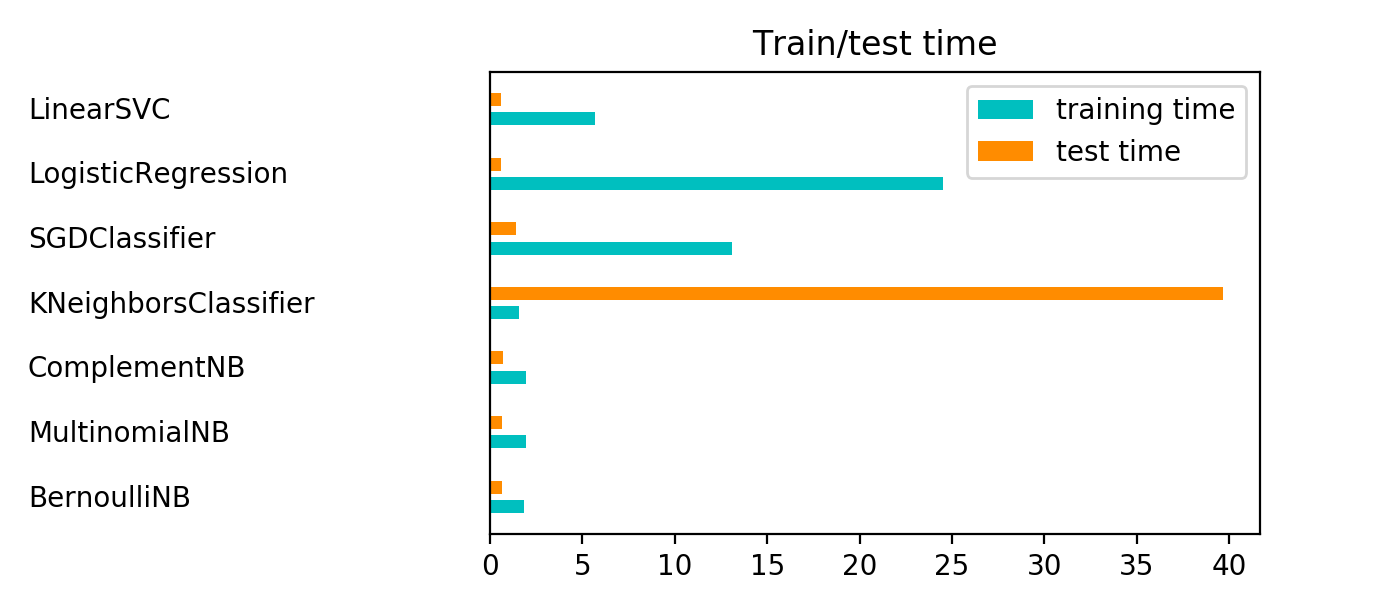
\includegraphics[width=\textwidth/2]{images/timing.png}
    \caption{Run-times (s) of selected SciKit-learn models.}
    \label{fig:runtimes}
\end{figure}

%%%%%%%%%%%%%%%%%%%%%%%%%%%%%%%%%%%%%%%%%%%%%%%%%%%%%%%%%%%%%%%%%%%%%%%%%%%%%%%%
\section{Discussion and Conclusion}

While our own Na\"ive Bayes implementation did not turn out to be very successful, we had a moderate amount of success with the scikit-learn models, especially when we evaluated their predictions together using an ensemble method. The scikit-learn Complement NB model, whose predictions had an accuracy of roughly $56\%$ was our best model when run independently, but we did have other models who were very close to this score.  The scikit-learn package's logistic regression model, multinomial Na\"ive Bayes model, and support vector machine model, all had accuracies in the mid 50s when run on their own. 

When weighted together in ensemble 'soft' voting, our models did even better. The voting allowed for an average accuracy of several methods to be leveraged together using a confidence-weighted majority vote to get a final total accuracy for the combination of models. Our best total accuracy came from the grouping of Logistic regression, Complement Na\"ive Bayes and Multinomial Na\"ive Bayes as predictors, which together reached an accuracy of 57.955\% (on the public leaderboard).

During our project we also discovered that---contrary to our expectations---the \texttt{PorterStemmer} pre-processing method was far more effective in terms of final prediction compared to the \texttt{WordNet} Lemmatization, and was far faster. In addition, we found that the more strict 'hard' ensemble vote, which takes predictions from each model as a binary, was less effective than the more relaxed average taken by the 'soft' ensemble vote.  

\subsection{Possible directions for future investigation}
One possible direction to go which we might try if we wished to design a different type of model that would be better able to extract the relevant data from these text comments would be to make use of pre-trained word embeddings.  Word embeddings are functions from the vocabulary to a vector space (usually of somewhere from 50-500 dimensions).  The idea behind such embeddings is that, once trained, they map similar words to similar vectors, and then they could be useful for this task since the features for a given text could be computed by combining these word embeddings.  A first example would be to just take the average of all the words in a comment, getting a comment-embedding, and use this as our pipeline for feature extraction.  However this would be ignoring a lot of information that the order of words contributes.

A better way to use pre-trained embeddings would be to use the embeddings in a neural network setup: we could implement a recurrent neural network (such as an LSTM), with the embeddings as a first layer, and a softmax for classification.\footnote{Still better results would surely be possible using pre-trained \textit{contextual} word embeddings such as generated by BERT\cite{devlin2018bert} or ELMo\cite{Peters:2018}, however this would certainly be beyond our current capability. Hopefully we will get there this semester.}

Going down this path seemed beyond the scope of this project at this point, and we chose to focus on the experimenting with the SciKit learn classifier models instead, though we remain curious as to whether we could have achieved a significant increase in performance with a more complicated neural network setup.

\subsection{Further questions}

While working to fine tune the models in order to achieve the best possible accuracy, we noticed that several models had better performance on certain specific classes. We could work to develop a more customized voting process to take into account the strengths/weaknesses of classifiers it contained, distributing weight during voting based on the class-specific precision of each algorithm. Or, noting  that all the models did rather poorly with comments from the community \textbf{r/funny}, but sklearn's Bernoulli NB in particular predicted that category relatively frequently for all validation comments, it would have been possibly useful to down-weight Bernoulli NB's vote if it was cast for \textbf{r/funny}.

%%%%%%%%%%%%%%%%%%%%%%%%%%%%%%%%%%%%%%%%%%%%%%%%%%%%%%%%%%%%%%%%%%%%%%%%%%%%%%%%
\section{Statement of contribution.}

The data processing was mainly coded and tested by Jacob and Orla. The SciKit learn models development and the hyperparameter testing were mostly done by Jacob and Lambert. Lambert developed our implementation of Bernoulli Na\"ive Bayes. A good part of the write up was done by Orla, and Jacob. 

%%%%%%%%%%%%%%%%%%%%%%%%%%%%%%%%%%%%%%%%%%%%%%%%%%%%%%%%%%%%%%%%%%%%%%%%%%%%%%%%
\bibliographystyle{abbrv}
\bibliography{cites}
\nocite{*}
\clearpage
\end{document}
